% !TEX root = ../00_tcc.tex

\begin{figure}[h]
	\centering
	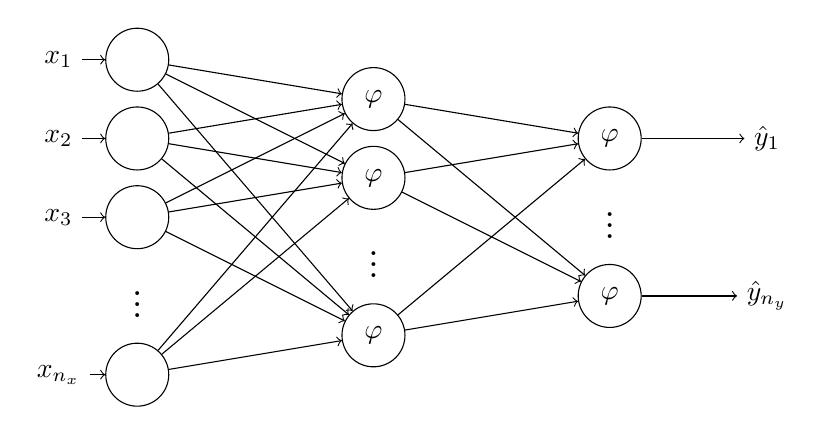
\begin{tikzpicture}
    \tikzstyle{neuron}=[circle, draw=black, minimum size = 8mm]

	\node[] (inp1)  at  (-4,2)   {$x_1$};
	\node[] (inp2)  at  (-4,1)   {$x_2$};
	\node[] (inp3)  at  (-4,0)   {$x_3$};
	\node[] (inp5)  at  (-4,-2)  {$x_{n_x}$};

	\node[neuron] (lay11)  at  (-3,2)   {};
	\node[neuron] (lay12)  at  (-3,1)   {};
	\node[neuron] (lay13)  at  (-3,0)   {};
	\node[]       (lay14)  at  (-3,-1)  {\Large$\vdots$};
	\node[neuron] (lay15)  at  (-3,-2)  {};

	\node[neuron] (lay21)  at  (0,1.5)   {$\varphi$};
	\node[neuron] (lay22)  at  (0,0.5)   {$\varphi$};
	\node[]       (lay23)  at  (0,-0.5)  {\Large$\vdots$};
	\node[neuron] (lay24)  at  (0,-1.5)  {$\varphi$};

	\node[neuron] (out1)    at  (3,1)   {$\varphi$};
	\node[]                 at  (3,0)   {\Large$\vdots$};
	\node[neuron] (out2)    at  (3,-1)  {$\varphi$};

	\node[]       (resul1)  at  (5,1)   {$\hat{y}_1$};
	\node[]       (resul2)  at  (5,-1)  {$\hat{y}_{n_y}$};

	\draw[->]  (out1)  --  (resul1)  ;
	\draw[->]  (out2)  --  (resul2)  ;

	\foreach \i in {1,2,3,5}{
		\draw[->]  (inp\i)  --  (lay1\i)  ;
		\foreach \j in {1,2,4}{
			\draw[->]  (lay1\i)  --  (lay2\j)  ;
		}
	}

	\foreach \i in {1,2,4}{
		\draw[->]  (lay2\i)  --  (out1)  ;
		\draw[->]  (lay2\i)  --  (out2)  ;
	}

	\end{tikzpicture}
	\caption{Representação de uma Rede Neural de 3 camadas, 1 oculta. Fonte: própria.}\label{tikz:nn}
\end{figure}
